\section*{Abstract}
Autonomous Unmanned Aerial Vehicle (UAV) swarms are increasingly adopted in mission-critical operations such as disaster response and large-scale environmental monitoring. However, deploying large Artificial Intelligence (AI) models on UAV platforms is constrained by strict Size, Weight, and Power (SWaP) limits, while cloud offloading introduces latency and connectivity dependencies that are often unacceptable in remote or contested environments.

This study formulates a joint Collaborative Edge Inference (CEI) optimization problem for deep learning inference distributed across heterogeneous UAV nodes connected through volatile Flying Ad-Hoc Networks (FANETs) \cite{matsubara2022split,mao2017mec}. The core technical challenge is \emph{computation--communication coupling}: partition boundaries determine intermediate tensor sizes, which in turn govern transmission delay and Radio Frequency (RF) energy consumption. We address this through a bounded-$K$ partitioning model with simultaneous optimization of partition selection and UAV assignment under coupled latency--energy objectives and SWaP constraints. Because the optimal solution depends on time-varying link quality, residual energy, and topology, we further develop online re-optimization mechanisms to preserve near-optimal performance and service continuity under dynamic swarm conditions. This work contributes analytical insight into the structure of the coupled optimization problem and provides empirical validation through network--robotics co-simulation.

\textbf{Index Terms---}Collaborative edge inference, UAV swarms, split inference, FANET, fault tolerance, resource-aware orchestration.

\begin{figure}[htbp]
  \centering
  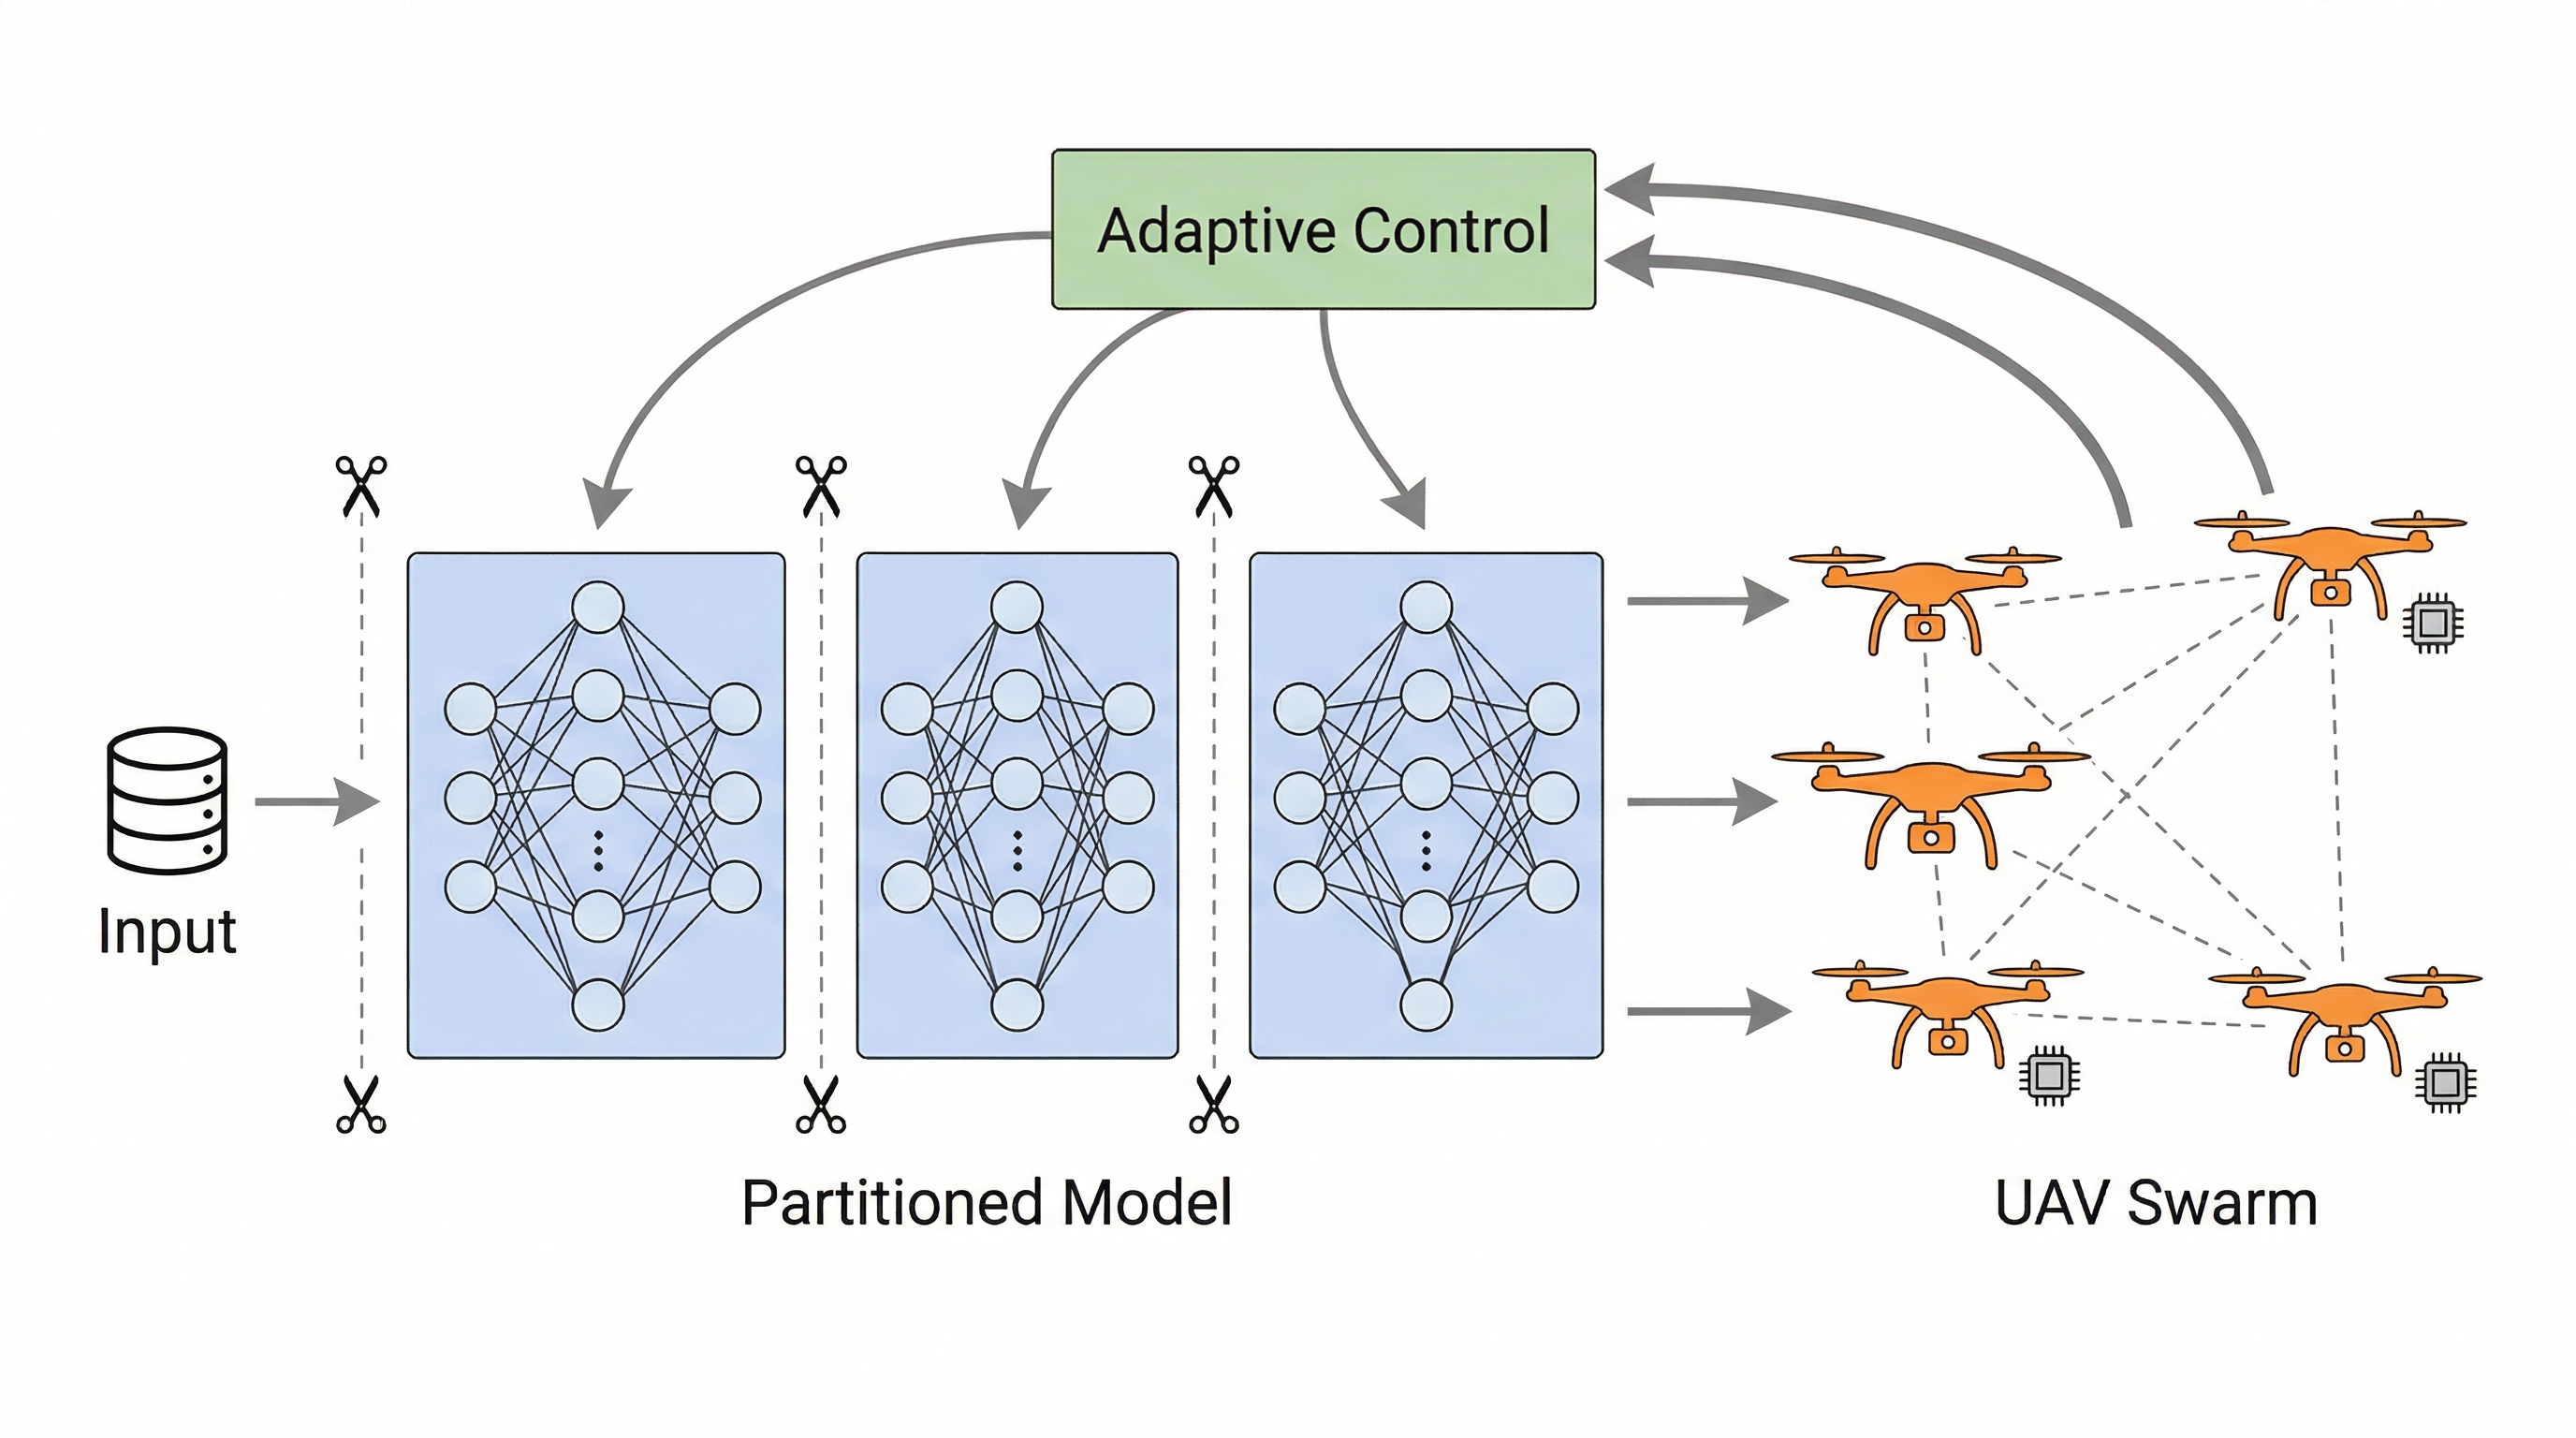
\includegraphics[width=0.90\linewidth]{image/graphical_abstract.png}
  \caption{Graphical abstract of the proposed three-layer CEI architecture for UAV swarms.}
  \label{fig:graphical_abstract}
\end{figure}
